\chapter{Machine Learning on Signals}

For most of this book we built filters and transforms by hand. We knew, from the
physics and the geometry, exactly what to compute: a band-pass to isolate a rhythm, a
spectrogram to watch frequencies move, an envelope to track muscle effort. That
hand-design works well when we understand the signal. But the wrist controller
we are building has to answer a messier question: \emph{which gesture is this?} The map
from a window of accelerometer and EMG samples to the label ``pinch'' or ``fist'' or
``rest'' is not a clean formula. It is a tangled boundary in a high-dimensional space,
different for every person's anatomy, drifting as the band slips on the arm. Nobody can
write that boundary down by hand.

So we let a model \emph{learn} it from examples. This chapter is about that move: from
features we compute (Chapters~27 and~38) to a decision rule fit to data.
We will keep the geometry front and center -- a classifier is a way of carving
feature space into regions -- and we will be direct about the two problems
that most often break real gesture systems: \emph{overfitting} (a model that memorizes its training
people instead of learning the gesture) and the \emph{cross-subject gap} (a model that
works on you and fails on everyone else). We end on the constraints that matter when the
model has to run inside a coin-cell-powered microcontroller strapped to a wrist.

This chapter is a tour, not a prerequisite. The wrist controller we build in the capstone
does not rely on a learned model: it uses direct per-finger calibration and template
matching, which are simpler to reason about and need no training set. Read this chapter to
understand what machine learning buys you and what it costs, so you can decide when it is
worth reaching for. For our build, it usually is not.

This chapter draws directly on the mathematical foundations in Chapter~42: probability gives us the language of
distributions, expectation, and generalization, while linear algebra gives us inner products
and the geometry of decision boundaries.

\section{Classification as carving up feature space}
\label{ch39:carving}

Suppose the feature extractor of the previous chapter has already turned each one-second
window of sensor data into a vector $\vec{x} \in \R^d$. A typical IMU window might give
$d \approx 20$ numbers: mean and variance of each accel axis, dominant frequency,
spectral energy in a few bands, the correlation between axes, and so on. Each window is
now a single \emph{point} in a $d$-dimensional space. A gesture, repeated many times,
produces a \emph{cloud} of points -- never identical, because of jitter, noise, and the
fact that you never make a fist exactly the same way twice. Figure~\ref{ch39:fig-imu-trace}
shows where one such point comes from: a raw sensor trace, a window, a few numbers.

\begin{figure}[H]
\centering
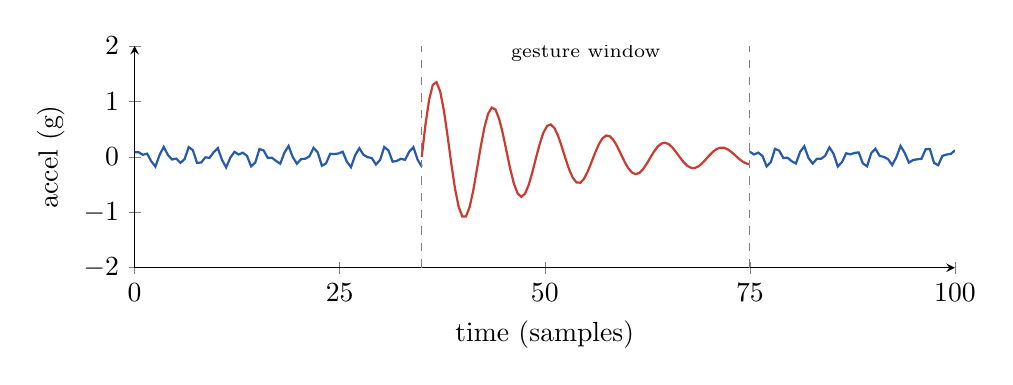
\begin{tikzpicture}
\begin{axis}[
  width=12cm, height=4.4cm,
  xlabel={time (samples)}, ylabel={accel (g)},
  domain=0:100, samples=160,
  xmin=0, xmax=100, ymin=-2, ymax=2,
  axis lines=left, xtick={0,25,...,100}, ytick={-2,-1,...,2},
  enlargelimits=false,
]
% rest region: small noise
\addplot[sigblue, thick, domain=0:35, samples=70]
  {0.12*sin(deg(2.1*x)) + 0.08*cos(deg(3.7*x))};
% gesture burst: a damped oscillation (a "wave")
\addplot[specred, thick, domain=35:75, samples=90]
  {1.5*exp(-0.06*(x-35))*sin(deg(0.9*(x-35)))};
% rest again
\addplot[sigblue, thick, domain=75:100, samples=50]
  {0.12*sin(deg(2.1*x)) + 0.08*cos(deg(3.7*x))};
\draw[gray, dashed] (axis cs:35,-2) -- (axis cs:35,2);
\draw[gray, dashed] (axis cs:75,-2) -- (axis cs:75,2);
\node[anchor=south, font=\scriptsize] at (axis cs:55,1.55) {gesture window};
\end{axis}
\end{tikzpicture}
\caption{A one-axis accelerometer trace: quiet rest (blue) bracketing a ``wave'' burst
(red). The feature extractor turns the boxed window into a handful of numbers -- its
energy, dominant frequency, and so on -- which become one point in feature space.}
\label{ch39:fig-imu-trace}
\end{figure}

\begin{intuitionbox}
Forget twenty dimensions for a moment and picture two features on a sheet of paper:
horizontal axis = signal energy, vertical axis = dominant frequency. ``Rest'' windows
cluster in the bottom-left (low energy, low frequency). ``Wave'' windows scatter
top-right (high energy, a clear oscillation). Classification amounts to
\emph{drawing a line (or curve) on this sheet} so that new points land on the correct
side. Everything else in this chapter is about how to draw that line well, in spaces
too high-dimensional to sketch.
\end{intuitionbox}

\begin{figure}[H]
\centering
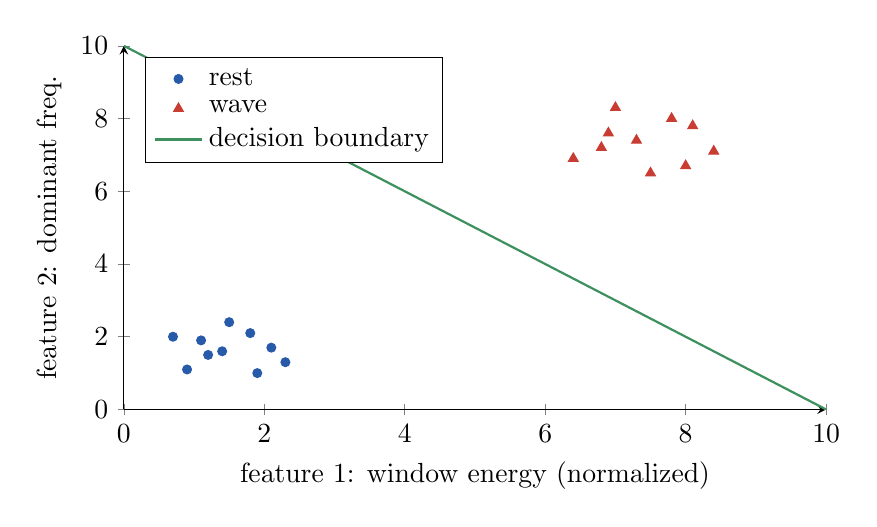
\begin{tikzpicture}
\begin{axis}[
  width=10.5cm, height=6.2cm,
  xlabel={feature 1: window energy (normalized)},
  ylabel={feature 2: dominant freq.},
  xmin=0, xmax=10, ymin=0, ymax=10,
  axis lines=left, xtick={0,2,...,10}, ytick={0,2,...,10},
  legend pos=north west, legend cell align=left,
  enlargelimits=false,
]
% rest cluster (bottom-left)
\addplot[only marks, mark=*, mark size=1.6pt, sigblue]
  coordinates {(1.2,1.5)(1.8,2.1)(0.9,1.1)(2.1,1.7)(1.5,2.4)(1.1,1.9)(2.3,1.3)(0.7,2.0)(1.9,1.0)(1.4,1.6)};
\addlegendentry{rest}
% wave cluster (top-right)
\addplot[only marks, mark=triangle*, mark size=2.0pt, specred]
  coordinates {(6.8,7.2)(7.5,6.5)(8.1,7.8)(7.0,8.3)(6.4,6.9)(8.4,7.1)(7.8,8.0)(6.9,7.6)(8.0,6.7)(7.3,7.4)};
\addlegendentry{wave}
% a separating line
\addplot[targetgreen, thick, domain=0:10, samples=2] {10-x};
\addlegendentry{decision boundary}
\end{axis}
\end{tikzpicture}
\caption{Two gesture classes as point clouds in a 2-D feature space. A classifier
draws the green boundary; new windows are labeled by which side they fall on. Real
problems live in $\R^{20}$ or higher, but the picture is the same.}
\label{ch39:fig-feature-space}
\end{figure}

\begin{connectionbox}
A feature vector $\vec{x}$ is a point in $\R^d$ equipped with an inner product (Chapter~42). A linear decision boundary is the set
$\set{\vec{x} : \inner{\vec{w}}{\vec{x}} + b = 0}$ -- a hyperplane, the level set of a
linear functional. The weight vector $\vec{w}$ is its normal direction. Classification
geometry \emph{is} the geometry of hyperplanes and projections.
\end{connectionbox}

\section{Logistic regression: a soft hyperplane}
\label{ch39:logistic}

The simplest useful classifier draws a single flat boundary -- a hyperplane -- and asks
which side a point is on. But a hard ``side'' gives no sense of confidence: a window
parked right on the boundary should not be reported with the same certainty as one deep
in fist territory. \emph{Logistic regression} fixes this by turning distance-from-the-
boundary into a probability.

We compute a linear score, the signed distance (up to scale) from the hyperplane,
\[
  z \;=\; \inner{\vec{w}}{\vec{x}} + b \;=\; \sum_{i=1}^{d} w_i x_i + b,
\]
and squash it through the \emph{logistic (sigmoid)} function
\[
  \sigma(z) \;=\; \frac{1}{1 + e^{-z}} \;\in\; (0,1),
\]
which we read as the model's estimated probability that the window is the positive class:
$\hat{p} = P(y{=}1 \mid \vec{x}) = \sigma(z)$.

\begin{figure}[H]
\centering
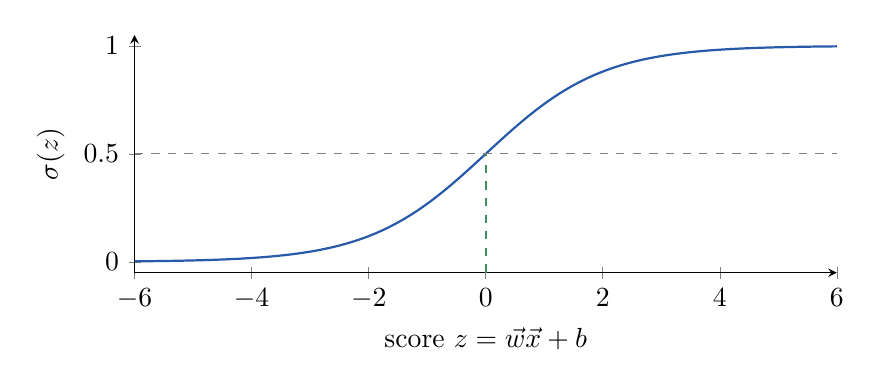
\begin{tikzpicture}
\begin{axis}[
  width=10.5cm, height=4.6cm,
  xlabel={score $z=\inner{\vec{w}}{\vec{x}}+b$}, ylabel={$\sigma(z)$},
  domain=-6:6, samples=120,
  xmin=-6, xmax=6, ymin=-0.05, ymax=1.05,
  axis lines=left, ytick={0,0.5,1}, xtick={-6,-4,...,6},
  enlargelimits=false,
]
\addplot[sigblue, thick] {1/(1+exp(-x))};
\addplot[gray, dashed, domain=-6:6, samples=2] {0.5};
\draw[targetgreen, thick, dashed] (axis cs:0,-0.05) -- (axis cs:0,0.5);
\end{axis}
\end{tikzpicture}
\caption{The logistic function maps any real score to a probability in $(0,1)$. At the
boundary ($z=0$) the model is maximally unsure ($\hat{p}=0.5$); far from it, the
probability saturates toward $0$ or $1$.}
\label{ch39:fig-sigmoid}
\end{figure}

\begin{whybox}
\textbf{Why the sigmoid, and what is the geometry of the covariance matrix?}
If you model each gesture class as a Gaussian cloud with mean $\vec{\mu}_k$ and shared
covariance matrix $\mat{\Sigma}$, Bayes' rule yields the logistic sigmoid
$\sigma(\vec{w}^\top\vec{x}+b)$ with exact linear arguments $\vec{w} = \mat{\Sigma}^{-1}(\vec{\mu}_1-\vec{\mu}_0)$.
To see why, take the log of the likelihood ratio. Each Gaussian contributes
$-\tfrac12(\vec{x}-\vec{\mu}_k)^\top\mat{\Sigma}^{-1}(\vec{x}-\vec{\mu}_k)$, and expanding
it gives $-\tfrac12\vec{x}^\top\mat{\Sigma}^{-1}\vec{x} + \vec{\mu}_k^\top\mat{\Sigma}^{-1}\vec{x} + (\text{const})$.
Because $\mat{\Sigma}$ is shared, the quadratic term $-\tfrac12\vec{x}^\top\mat{\Sigma}^{-1}\vec{x}$
is identical for both classes and cancels in the difference, leaving the log-odds
$(\vec{\mu}_1-\vec{\mu}_0)^\top\mat{\Sigma}^{-1}\vec{x} + b$, linear in $\vec{x}$ (the
constants and the log prior ratio collect into $b$). Bayes' rule turns log-odds $z$
into the probability $1/(1+e^{-z}) = \sigma(z)$.

The covariance matrix $\mat{\Sigma} = \mathbb{E}[(\vec{x}-\vec{\mu})(\vec{x}-\vec{\mu})^\top]$
encodes the geometric shape and orientation of the point cloud. Because $\mat{\Sigma}$ is
symmetric and positive-definite, its eigendecomposition $\mat{\Sigma} = \mat{V}\mat{\Lambda}\mat{V}^\top$
aligns with the cloud's principal axes: the orthonormal eigenvectors $\vec{v}_i$ define the
directions of tilt, and the eigenvalues $\lambda_i = \sigma_i^2$ give the variance along each axis.
Contour curves of equal probability density are ellipsoids satisfying
$(\vec{x}-\vec{\mu})^\top \mat{\Sigma}^{-1} (\vec{x}-\vec{\mu}) = c^2$.
The quantity $d_M(\vec{x},\vec{\mu}) = \sqrt{(\vec{x}-\vec{\mu})^\top \mat{\Sigma}^{-1} (\vec{x}-\vec{\mu})}$
is the \textbf{Mahalanobis distance}: it measures distance in units of standard deviation along
the cloud's natural axes. Standard Euclidean distance implicitly assumes $\mat{\Sigma}=\mat{I}$
(an isotropic spherical cloud); taking the true covariance into account un-distorts the feature
space, preventing high-variance noise features from drowning out subtle gesture cues.
\end{whybox}

\subsection{Training: maximize the probability of the data}
\label{ch39:logistic-train}

We have parameters $\vec{w}, b$ and a labeled training set
$\set{(\vec{x}^{(n)}, y^{(n)})}_{n=1}^{N}$ with $y^{(n)} \in \set{0,1}$. We pick the
parameters that make the observed labels most probable. The probability the model
assigns to one example is $\hat{p}^{\,y}(1-\hat{p})^{1-y}$, and assuming independent
examples, the log-likelihood of the whole set is a sum. Maximizing it is the same as
minimizing the average \emph{cross-entropy loss}
\[
  L(\vec{w},b) \;=\; -\frac{1}{N}\sum_{n=1}^{N}
     \Big[\, y^{(n)} \log \hat{p}^{(n)} \;+\; (1-y^{(n)}) \log\!\big(1-\hat{p}^{(n)}\big) \,\Big].
\]
There is no closed-form minimizer, so we use \emph{gradient descent}: nudge the
parameters downhill on $L$. The gradient has a simple form,
\[
  \frac{\partial L}{\partial \vec{w}}
   \;=\; \frac{1}{N}\sum_{n=1}^{N} \big(\hat{p}^{(n)} - y^{(n)}\big)\,\vec{x}^{(n)},
\]
i.e.\ average the input vectors weighted by the prediction error. The simplicity comes
from a cancellation. For one example with score $z=\vec{w}^\top\vec{x}+b$, the sigmoid's
slope is $\sigma'(z) = \hat{p}(1-\hat{p})$, and the chain rule gives
\[
  \frac{\partial L}{\partial z}
  = -\Big(\frac{y}{\hat{p}} - \frac{1-y}{1-\hat{p}}\Big)\,\hat{p}(1-\hat{p})
  = -\big(y(1-\hat{p}) - (1-y)\hat{p}\big) = \hat{p} - y ,
\]
the denominators of the log-loss cancelling against the sigmoid's slope; multiplying by
$\partial z/\partial\vec{w} = \vec{x}$ gives the formula above. Each step moves the
boundary to reduce its mistakes.

\begin{connectionbox}
That gradient is just the multivariable chain rule (Chapter~42) applied to a composition
$L \circ \sigma \circ (\text{linear})$, and the loss is the negative log-likelihood derived from independent trials.
\end{connectionbox}

\begin{example}[Logistic boundary by hand]
\label{ch39:ex-logistic}
Take one feature, EMG envelope energy $x$, and two classes: rest ($y{=}0$) and
clench ($y{=}1$). Suppose after training $w = 1.5$, $b = -6$, so $z = 1.5x - 6$. The
boundary $z=0$ sits at $x = 4$. A window with $x=5$ gives $z=1.5$, so
$\hat{p}=\sigma(1.5)\approx 0.82$ -- ``probably a clench.'' A window with $x=4.2$ gives
$z=0.3$, $\hat{p}\approx 0.57$ -- barely past the line, low confidence. The slope $w$
controls how fast confidence rises as you move away from $x=4$; a larger $w$ makes a
sharper, more decisive boundary.
\end{example}

\subsection{Regularization: the first guard against overfitting}
\label{ch39:reg}

If a feature happens to separate the training set perfectly, gradient descent will push
its weight toward infinity to make $\hat{p}$ hit exactly $0$ or $1$ -- overconfident
predictions based on a coincidence in the training data. We discourage this by adding a penalty on large weights,
typically the $L_2$ term $\tfrac{\lambda}{2}\norm{\vec{w}}^2$, to the loss. This
\emph{regularization} keeps the weights small and the predicted probabilities moderate; $\lambda$ is
a knob we tune on validation data (Section~\ref{ch39:eval}). It is our first concrete
defense against overfitting.

\section{Support vector machines: maximizing the margin}
\label{ch39:svm}

Logistic regression will accept any separating hyperplane that lowers the loss. But if
two classes are cleanly separated, infinitely many hyperplanes separate them -- which is
best? The \emph{support vector machine} (SVM) gives a geometric answer: choose the
boundary that leaves the \emph{widest empty margin} between the classes, the one that
stays as far as possible from the nearest points of both clouds.

\begin{figure}[H]
\centering
\begin{tikzpicture}[font=\small, scale=0.88, every node/.style={transform shape}, >=Latex]
  \definecolor{sigblue}{RGB}{40,90,170}
  \definecolor{specred}{RGB}{200,60,50}
  \definecolor{targetgreen}{RGB}{62,145,95}

  % Panel A: Maximum Margin Linear SVM
  \begin{scope}[shift={(0,0)}]
    \node[font=\footnotesize\bfseries, anchor=south] at (2.4, 4.8) {Linear SVM: Maximum-Margin Separator};
    \draw[->, gray!60] (0,0) -- (5.0,0) node[right, font=\scriptsize] {$x_1$ (energy)};
    \draw[->, gray!60] (0,0) -- (0,3.8) node[left, font=\scriptsize] {$x_2$};

    % Margin corridor fill
    \fill[green!8] (0.2, 0.4) -- (0.2, 1.8) -- (4.4, 4.32) -- (4.4, 2.92) -- cycle;

    % Class 1 (Rest: Blue)
    \foreach \p in {(0.8, 1.8), (1.2, 2.5), (1.5, 1.2), (0.6, 2.7), (2.0, 2.3)} {
      \fill[sigblue] \p circle (2pt);
    }
    \coordinate (SV1) at (2.2, 3.0);
    \fill[sigblue] (SV1) circle (2pt);
    \draw[sigblue, thick] (SV1) circle (4pt);

    % Class 2 (Gesture: Red)
    \foreach \p in {(3.2, 0.6), (3.8, 1.4), (4.2, 0.8), (3.6, 2.0), (4.4, 1.8)} {
      \fill[specred] \p circle (2pt);
    }
    \coordinate (SV2) at (2.4, 1.72);
    \fill[specred] (SV2) circle (2pt);
    \draw[specred, thick] (SV2) circle (4pt);
    \coordinate (SV3) at (3.4, 2.32);
    \fill[specred] (SV3) circle (2pt);
    \draw[specred, thick] (SV3) circle (4pt);

    % Decision boundary
    \draw[targetgreen, very thick] (0.2, 1.1) -- (4.4, 3.62) node[above, font=\tiny\bfseries] {$\vec{w}^\top\vec{x}+b=0$};
    \draw[targetgreen, dashed, thick] (0.2, 1.8) -- (4.2, 4.12) node[pos=0.8, above left, font=\tiny] {$\vec{w}^\top\vec{x}+b=+1$};
    \draw[targetgreen, dashed, thick] (0.2, 0.4) -- (4.4, 2.92) node[below right, font=\tiny] {$\vec{w}^\top\vec{x}+b=-1$};

    % Margin width dimension line
    \draw[<->, black, thick] (1.3, 2.45) -- (2.0, 1.3) node[midway, left=5pt, font=\tiny\bfseries] {$\text{Margin} = \frac{2}{\|\vec{w}\|}$};

    % Weight normal vector
    \draw[->, ultra thick, targetgreen!80!black] (2.3, 2.36) -- ++(-0.6, 1.0) node[above left, font=\tiny] {$\vec{w}$ (normal)};
  \end{scope}

  % Panel B: Non-linear RBF Kernel Boundary
  \begin{scope}[shift={(7.5,0)}]
    \node[font=\footnotesize\bfseries, anchor=south] at (2.4, 4.8) {Kernel SVM: Non-Linear Boundary};
    \draw[->, gray!60] (0,0) -- (5.0,0) node[right, font=\scriptsize] {$x_1$};
    \draw[->, gray!60] (0,0) -- (0,3.8) node[left, font=\scriptsize] {$x_2$};

    % Inner cluster (Rest: Blue)
    \foreach \p in {(2.4, 2.1), (2.1, 2.4), (2.6, 2.4), (2.3, 1.8), (2.7, 1.9)} {
      \fill[sigblue] \p circle (2pt);
    }
    % Outer ring cluster (Flick: Red)
    \foreach \ang in {20, 60, 100, 140, 180, 220, 260, 300, 340} {
      \fill[specred] (2.4, 2.1) ++(\ang:1.6) circle (2pt);
    }

    \draw[targetgreen, very thick] (2.4, 2.1) circle (1.1);
    \node[targetgreen!80!black, font=\tiny\bfseries, anchor=north] at (2.4, 0.9) {RBF Boundary};
    \node[font=\scriptsize, align=center, text=gray!80!black] at (2.4, -0.6) 
      {Mapped implicitly to higher dimension;\\linear hyperplanes cannot separate rings};
  \end{scope}
\end{tikzpicture}
\caption{Geometry of Support Vector Machines. Left: linear SVM maximizes the margin corridor $\frac{2}{\|\vec{w}\|}$ between classes; only the circled support vectors touching the gutters define the decision boundary $\vec{w}^\top\vec{x}+b=0$. Right: when gesture classes form non-linear topologies (e.g.\ an inner rest cluster surrounded by an energetic movement ring), the kernel trick implicitly lifts points into an inner-product Hilbert space where a smooth boundary is found without computing high-dimensional coordinates.}
\label{ch39:fig-svm}
\end{figure}

The distance from a point to the hyperplane $\inner{\vec{w}}{\vec{x}}+b=0$ is
$\abs{\inner{\vec{w}}{\vec{x}}+b}/\norm{\vec{w}}$. Fixing the scale so the closest points
satisfy $\abs{z}=1$, the margin half-width is $1/\norm{\vec{w}}$. Maximizing the margin
therefore means \emph{minimizing} $\norm{\vec{w}}$ subject to every point being on the
correct side by at least the margin:
\[
  \min_{\vec{w},b}\ \tfrac12\norm{\vec{w}}^2
  \quad\text{s.t.}\quad
  y^{(n)}\big(\inner{\vec{w}}{\vec{x}^{(n)}}+b\big) \ge 1 \ \ \forall n,
\]
where labels are written as $y^{(n)}\in\set{-1,+1}$. Real data are not cleanly
separable, so we allow slack: points may sit inside the margin or on the wrong side, at
a cost. This gives the \emph{soft-margin} SVM, whose loss is the hinge loss
$\max(0,\,1 - y\,z)$ plus the same $\norm{\vec{w}}^2$ penalty -- again a margin-vs-
violations trade-off controlled by a knob $C$.

\begin{happeningbox}
Once the margin is set, only the support vectors (the few
points touching the gutter) matter; the rest of each cloud is irrelevant. This is the
opposite of logistic regression, which is nudged by \emph{every} point. For gesture
data with one dominant, well-separated rest class, the SVM's focus on the hard,
borderline windows is often exactly what you want.
\end{happeningbox}

\subsection{The kernel trick: curved boundaries from inner products}
\label{ch39:kernel}

\begin{historybox}
\textbf{Vladimir Vapnik, Structural Risk, and Mercer's Kernels (1995)}
For decades, pattern recognition was caught between two extremes: simple linear classifiers (like Frank Rosenblatt's 1958 Perceptron), which were mathematically transparent but could not separate non-linear topologies (the famous XOR problem demonstrated by Minsky and Papert in 1969); and multi-layer neural networks, which could learn non-linear curves but suffered from non-convex loss surfaces, unpredictable local minima, and vanishing gradients.

In 1995 at AT\&T Bell Laboratories, Soviet-American mathematician Vladimir Vapnik presented the \textbf{Support Vector Machine} (SVM). Vapnik realized that the optimal linear decision boundary is the unique hyperplane that maximizes the geometric \emph{margin} --- the buffer zone between classes. For data inside a ball of radius $R$, hyperplanes with margin at least $\Delta$ have Vapnik--Chervonenkis (VC) dimension at most about $R^2/\Delta^2$, regardless of the number of features, so maximizing the margin tightens a theoretical bound on overfitting.

To solve non-linear problems, Bernhard Boser, Isabelle Guyon, and Vapnik (1992) applied a theorem proved in 1909 by British mathematician James Mercer. Mercer's Theorem states that any continuous, symmetric, positive semi-definite function $k(\vec{x},\vec{x}')$ can be expanded as an inner product in some high-dimensional (and potentially infinite-dimensional) Hilbert space:
\[
  k(\vec{x},\vec{x}') \;=\; \inner{\phi(\vec{x})}{\phi(\vec{x}')}_{\mathcal{H}}.
\]
This yielded the famous \textbf{``kernel trick''}: an SVM's dual quadratic programming optimization depends \emph{only} on pairwise inner products between data points. By replacing $\inner{\vec{x}}{\vec{x}'}$ with a Mercer kernel like the Radial Basis Function (RBF), the SVM implicitly projects raw feature vectors into an infinite-dimensional space where gesture clusters that are tangled in the original space can become linearly separable, \emph{without ever computing or storing the infinite-dimensional coordinates}.
\end{historybox}

\begin{trapbox}
\textbf{Raw Signal Vectors and the Curse of Dimensionality}
A frequent temptation for modern practitioners is: ``Why spend time engineering DSP features? Let's just flatten the raw sensor stream into a vector and feed it directly into an ML classifier!''

Consider the numbers: an IMU streaming 6 axes ($a_x, a_y, a_z, g_x, g_y, g_z$) across a modest $400\,\text{ms}$ window at $200\,\text{Hz}$ produces $80$ time steps per axis. Flattening this array yields an input vector of dimension:
\[
  D \;=\; 6 \;\times\; 80 \;=\; \mathbf{480 \text{ dimensions}}.
\]
In a 480-dimensional space, learning hits Richard Bellman's (1957) \textbf{Curse of Dimensionality}:
\begin{enumerate}
  \item \emph{Exponential Sparsity:} The volume of a hypercube scales as $L^D$. To sample a 480-dimensional space with the same density as just 10 points along a 1D line would require $10^{480}$ training gestures --- more than the number of atoms in the observable universe.
  \item \emph{Distance Metric Collapse:} In high dimensions, the contrast between Euclidean distances vanishes: the ratio of the distance to the nearest neighbor versus the farthest neighbor approaches $1$ ($\lim_{D\to\infty} \frac{d_{\max} - d_{\min}}{d_{\min}} \to 0$). Every gesture looks equally far from every other gesture.
  \item \emph{Severe Overfitting:} With 480 dimensions and only a few dozen training examples, a classifier easily memorizes arbitrary high-frequency noise spikes, reaching $100\%$ training accuracy while failing on new gestures.
\end{enumerate}
\textbf{The DSP Solution:} Domain-specific feature engineering uses physical principles (Parseval energy, zero crossings, spectral centroids, auto-regressive coefficients) to project $\R^{480}$ down to an informative, compact $\R^{12}$ manifold. In 12 dimensions, clusters are dense, distances are meaningful, and models generalize reliably with small, lightweight training sets.
\end{trapbox}

A flat hyperplane cannot separate clouds that wrap around each other -- think ``slow
wrist roll'' versus ``fast wrist roll,'' where the deciding feature is a \emph{ring} in
feature space, not a half-plane. The kernel trick maps points into a higher-dimensional
space where they \emph{do} separate linearly, without ever computing the map explicitly.
Because the SVM only ever needs inner products $\inner{\vec{x}}{\vec{x}'}$, we replace
them with a \emph{kernel} $k(\vec{x},\vec{x}')$ -- the inner product in the lifted space.
The popular radial basis function (RBF) kernel
\[
  k(\vec{x},\vec{x}') \;=\; \exp\!\big(-\gamma\,\norm{\vec{x}-\vec{x}'}^2\big)
\]
yields smooth, curved boundaries that bend around clusters. The price: an RBF-SVM must
store the support vectors and compute a kernel against each one at inference time, which
matters on a microcontroller (Section~\ref{ch39:ondevice}).

\section{Random forests: many simple questions}
\label{ch39:forests}

Linear and kernel methods think in terms of distances and dot products. A \emph{decision
tree} thinks in terms of yes/no questions about one feature at a time: ``Is the accel-z
variance above $0.4$? If yes, is the dominant frequency below $3$\,Hz?'' Each question
splits the data; following the branches leads to a leaf that votes for a class. A single
tree carves feature space into axis-aligned boxes.

A single deep tree overfits badly -- it will keep asking questions until every training
window sits alone in its own box. The \emph{random forest} tames this by averaging many
trees, each trained on a bootstrap resample of the data and allowed to consider only a
random subset of features at each split. The trees disagree in their mistakes but agree
on the real structure, so their majority vote is far more robust than any one tree.

\begin{figure}[H]
\centering
\begin{tikzpicture}[
  every node/.style={font=\scriptsize, align=center},
  box/.style={draw, rounded corners, fill=blue!4, inner sep=3pt},
  leaf/.style={draw, fill=green!6, inner sep=3pt}
]
\node[box] (root) {var$_z>0.4$?};
\node[box, below left=0.8cm and 1.1cm of root] (l) {freq$<3$?};
\node[leaf, below right=0.8cm and 1.1cm of root] (r) {wave};
\node[leaf, below left=0.7cm and 0.2cm of l] (ll) {rest};
\node[leaf, below right=0.7cm and 0.2cm of l] (lr) {hold};
\draw[->] (root) -- node[above left]{no} (l);
\draw[->] (root) -- node[above right]{yes} (r);
\draw[->] (l) -- node[left]{yes} (ll);
\draw[->] (l) -- node[right]{no} (lr);
\end{tikzpicture}
\caption{One small decision tree on IMU features. A random forest grows hundreds of
such trees on resampled data and votes; the diversity is what prevents any single tree's
overfitting from dominating.}
\label{ch39:fig-tree}
\end{figure}

\begin{whybox}
Why does averaging help? Each tree's prediction is a noisy estimate of the truth. If the
trees' errors were perfectly correlated, averaging would do nothing. Bootstrap sampling
and random feature subsets \emph{decorrelate} the errors, and the variance of an average
of $T$ weakly-correlated estimators shrinks roughly like $1/T$ plus a residual
correlation floor. This is the same variance-reduction-by-averaging law from Chapter~20 (and Chapter~42) for the sample mean -- applied to predictors instead of numbers.
\end{whybox}

\begin{aestheticbox}
Random forests are often the best first thing to try on hand-crafted signal
features. They need almost no feature scaling, tolerate irrelevant features,
handle nonlinear boundaries, rarely overfit catastrophically, and hand back an interpretable
\emph{feature-importance} ranking that shows which features actually carry predictive
weight. That ranking is a practical guide to trimming your feature set down to what fits on an MCU.
\end{aestheticbox}

\clearpage
\section{When to hand-craft features and when to learn them}
\label{ch39:features-vs-raw}

Everything above assumes someone already computed a good feature vector. Choosing those
features -- spectral energies, zero-crossing rates, axis correlations -- is itself a design
task, and it bakes in your understanding of the signal. That is a strength (you
inject physics) and a weakness (you might omit the very pattern that distinguishes two
gestures). Neural networks offer the alternative: feed the model something close to raw
samples and let it discover its own features.

\begin{trapbox}
``Deep learning means I can skip feature engineering'' is a tempting and expensive
mistake on small sensor datasets. With a few thousand labeled windows from a dozen
people, a random forest on well-chosen features will usually \emph{beat} a raw-window
neural net, train in seconds, and fit on the microcontroller. Raw-input nets pay off
when you have a lot of data and patterns too subtle to name. Know which regime you are
in before you reach for a deep network.
\end{trapbox}

\section{Small neural networks}
\label{ch39:mlp}

A neural network stacks the logistic idea. One \emph{neuron} computes a weighted sum and
a nonlinearity, $a = \phi(\inner{\vec{w}}{\vec{x}}+b)$; a \emph{layer} runs many neurons
in parallel; stacking layers lets later neurons build features out of earlier ones. With
just one hidden layer,
\[
  \vec{h} = \phi(\mat{W}_1\vec{x} + \vec{b}_1), \qquad
  \hat{\vec{p}} = \mathrm{softmax}(\mat{W}_2\vec{h} + \vec{b}_2),
\]
the network can represent boundaries no single hyperplane can. The nonlinearity $\phi$ is
essential: without it, stacking linear maps just gives another linear map. The modern
default is the \emph{ReLU}, $\phi(z)=\max(0,z)$ -- cheap to compute and cheap to
differentiate, which matters both for training speed and for MCU inference.

\begin{figure}[H]
\centering
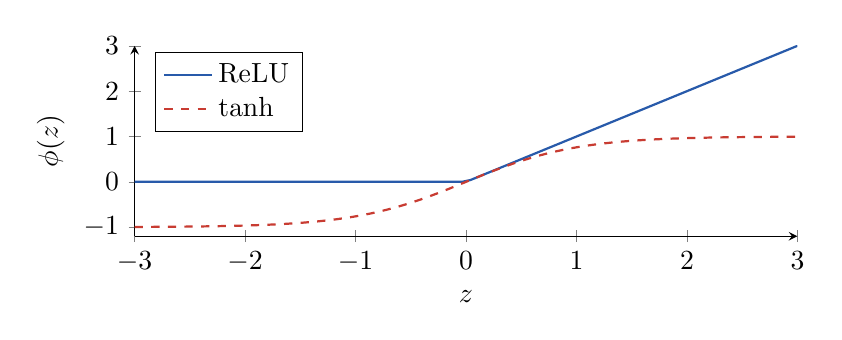
\begin{tikzpicture}
\begin{axis}[
  width=10cm, height=4cm,
  xlabel={$z$}, ylabel={$\phi(z)$},
  domain=-3:3, samples=80,
  xmin=-3, xmax=3, ymin=-1.2, ymax=3,
  axis lines=left, legend pos=north west, legend cell align=left,
  enlargelimits=false,
]
\addplot[sigblue, thick] {max(0,x)};
\addlegendentry{ReLU}
\addplot[specred, thick, dashed] {tanh(x)};
\addlegendentry{tanh}
\end{axis}
\end{tikzpicture}
\caption{Two common nonlinearities. The ReLU's flat-then-linear shape is fast and avoids
the saturation that slows learning; $\tanh$ is smooth but saturates at both ends.}
\label{ch39:fig-relu}
\end{figure}

\subsection{Softmax for several gestures}
\label{ch39:softmax}

Our controller has more than two gestures, so the output layer produces one score per
class and normalizes them into a probability distribution with the \emph{softmax}:
\[
  \hat{p}_k \;=\; \frac{e^{z_k}}{\sum_{j} e^{z_j}}, \qquad \sum_k \hat{p}_k = 1.
\]
Training minimizes multi-class cross-entropy, and the gradient is computed by
\emph{backpropagation} -- the chain rule run backward through the layers, reusing each
layer's stored output. It is the multivariable chain rule (Chapter~42), organized to avoid
recomputation.

\begin{trapbox}
A small net has lots of parameters relative to a small gesture dataset, so it overfits
even more eagerly than logistic regression. The standard countermeasures are
\emph{dropout} (randomly zero some hidden units during training, forcing redundancy),
weight decay (the same $L_2$ penalty), and \emph{early stopping} (halt when validation
loss stops improving). Use them; an unregularized net on a few thousand windows will
report near-perfect training accuracy and fail in the field.
\end{trapbox}

\section{1-D convolutional networks on raw windows}
\label{ch39:cnn}

Convolutional networks connect directly to the rest of the book. A convolutional
neural network does not invent a new operation -- its core layer is the \emph{convolution}
we spent whole chapters on. A 1-D CNN slides a short learnable filter (kernel) along the
raw signal window and records the response at each position, exactly like an FIR filter,
except the taps are \emph{learned} rather than designed.

\begin{happeningbox}
A hand-designed band-pass filter has fixed taps chosen so its frequency response passes
$8$--$12$\,Hz. A learned conv kernel has taps chosen by gradient descent to maximize
gesture-classification accuracy. The machinery is identical -- multiply, shift, add (the
convolution sum $\sum_k h[k]\,x[n-k]$) -- but the design objective moved from ``match this
frequency response'' to ``be useful for the task.'' A CNN is a stack of FIR filters whose
coefficients the data chooses.
\end{happeningbox}

A typical 1-D CNN for gestures looks like: a few conv layers (each a bank of short
learned filters followed by a ReLU), interleaved with \emph{pooling} that downsamples by
keeping the max in each small window (cheap translation tolerance, so a gesture detected
slightly early or late still fires), then a small dense head with a softmax. Because the
same kernel is reused at every position (\emph{weight sharing}), a CNN has far fewer
parameters than a dense net reading the same raw window -- a real advantage when data is
scarce and memory is tight.

\begin{figure}[H]
\centering
\begin{tikzpicture}[
  every node/.style={font=\scriptsize, align=center},
  blk/.style={draw, rounded corners, minimum height=1cm, minimum width=1.5cm},
]
\node[blk, fill=blue!4] (in) {raw window\\$3\times 50$};
\node[blk, fill=orange!6, right=0.45cm of in] (c1) {conv+ReLU\\8 filt., len 5};
\node[blk, fill=green!5, right=0.45cm of c1] (p1) {max-pool\\$/2$};
\node[blk, fill=orange!6, right=0.45cm of p1] (c2) {conv+ReLU\\16 filt.};
\node[blk, fill=gray!7, right=0.45cm of c2] (fc) {dense};
\node[blk, fill=violet!8, right=0.45cm of fc] (out) {softmax\\$K$ gestures};
\draw[->] (in)--(c1); \draw[->] (c1)--(p1); \draw[->] (p1)--(c2);
\draw[->] (c2)--(fc); \draw[->] (fc)--(out);
\end{tikzpicture}
\caption{A small 1-D CNN for gesture windows. Input is three accel axes $\times$ 50
samples. Early conv layers learn FIR-like filters; pooling adds time-shift tolerance;
the dense head maps learned features to gesture probabilities.}
\label{ch39:fig-cnn}
\end{figure}

\begin{goalbox}
Whatever classifier you choose, the sensor sets the ceiling. A wrist IMU sees \emph{gross
forearm motion}: a wave, a twist, a tap, a sharp flick. It does not see individual finger
joints -- those move with almost no signature at the wrist. If your gesture set is ``open
hand vs.\ closed fist held still,'' the IMU is nearly blind to it; you need EMG or
force-myography for finger-level discrimination (Chapter~37). A classifier
can only be as good as the information the sensor captured. This is exactly why our
capstone leans on per-finger sensing and calibration rather than on a learned model
guessing gestures from coarse wrist motion: improving the signal helps more than
changing the algorithm.
\end{goalbox}

\section{Evaluating without fooling yourself: train, validation, test}
\label{ch39:eval}

A model's accuracy on the data it was trained on is almost meaningless -- a lookup table
that memorizes the training set scores 100\% and learns nothing. What we care about is
\emph{generalization}: accuracy on windows the model has never seen. To estimate it we
split our data into three disjoint parts.

\begin{itemize}
  \item \textbf{Training set} -- used to fit the parameters $\vec{w},b,\mat{W}$.
  \item \textbf{Validation set} -- used to choose hyperparameters ($\lambda$, $C$,
        $\gamma$, number of trees, network size, when to stop). The model never trains on
        it, but \emph{you} tune against it, so it slowly leaks information.
  \item \textbf{Test set} -- touched exactly once, at the very end, to report true
        performance. If you peek at it while developing, it stops being a test set.
\end{itemize}

\begin{figure}[H]
\centering
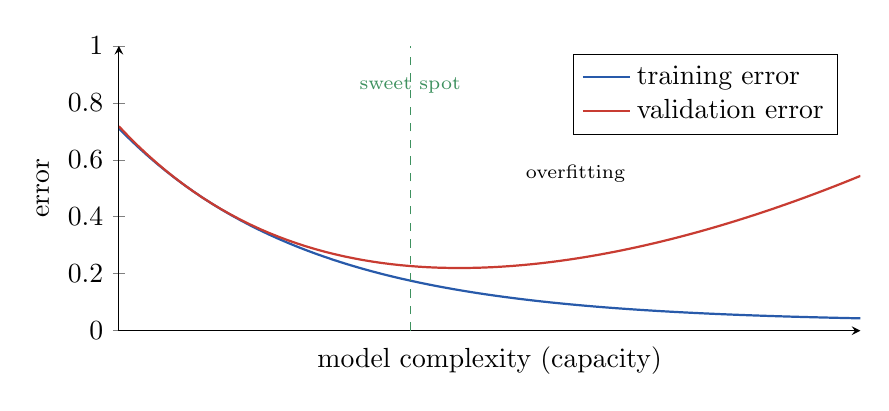
\begin{tikzpicture}
\begin{axis}[
  width=11cm, height=5.2cm,
  xlabel={model complexity (capacity)}, ylabel={error},
  domain=0.4:6, samples=80,
  xmin=0.4, xmax=6, ymin=0, ymax=1.0,
  axis lines=left, legend pos=north east, legend cell align=left,
  xtick=\empty,
  enlargelimits=false,
]
\addplot[sigblue, thick] {0.9*exp(-0.7*x)+0.03};
\addlegendentry{training error}
\addplot[specred, thick] {0.9*exp(-0.7*x)+0.03 + 0.02*(x-1)^2};
\addlegendentry{validation error}
\draw[targetgreen, dashed] (axis cs:2.6,0) -- (axis cs:2.6,1.0);
\node[targetgreen, anchor=south, font=\scriptsize] at (axis cs:2.6,0.80){sweet spot};
\node[anchor=west, font=\scriptsize] at (axis cs:3.4,0.55){overfitting};
\end{axis}
\end{tikzpicture}
\caption{The overfitting picture. As capacity grows, training error keeps falling but
validation error turns back up: the model starts memorizing noise. We pick the
complexity at the validation minimum, not the training minimum.}
\label{ch39:fig-overfit}
\end{figure}

\begin{whybox}
Overfitting is the central hazard, so it is worth saying precisely what it is. A flexible
model can fit the \emph{noise} in the training set -- the random jitter that will be
different next time -- as if it were signal. Statistical learning frames this as the
bias--variance trade-off: a too-simple model is biased (it cannot represent the truth),
a too-complex one has high variance (it swings wildly with the particular training
sample). Validation error is our empirical estimate of where that trade-off is best.
\end{whybox}

\subsection{Cross-validation when data is scarce}
\label{ch39:cv}

Gesture data is expensive: every window is someone making a gesture on cue. A single
fixed split then wastes data and gives a noisy estimate. \emph{$k$-fold cross-validation}
uses it all: partition into $k$ folds, train on $k-1$ and validate on the held-out fold,
rotate through all $k$ choices, and average. You get a more stable estimate and a sense
of its variance across folds.

\section{The cross-subject gap}
\label{ch39:cross-subject}

This is the most important point in this chapter, and the one most
often gotten wrong. \textbf{How you split matters more than the model.} If you pool all
windows from all people and split randomly, windows from the \emph{same person} -- even
the same recording session -- land in both train and test. The model can then succeed by
recognizing the \emph{person} (their arm shape, band placement, skin impedance, personal
style) rather than the \emph{gesture}. Your reported accuracy looks high and drops sharply
when a new user straps on the band.

The fix is \emph{cross-subject} (also called leave-one-subject-out) evaluation: hold out
\emph{all} data from some people, train on the rest, test on the held-out strangers.
This measures what we actually care about -- does the system work on a person it has
never seen?

\begin{figure}[H]
\centering
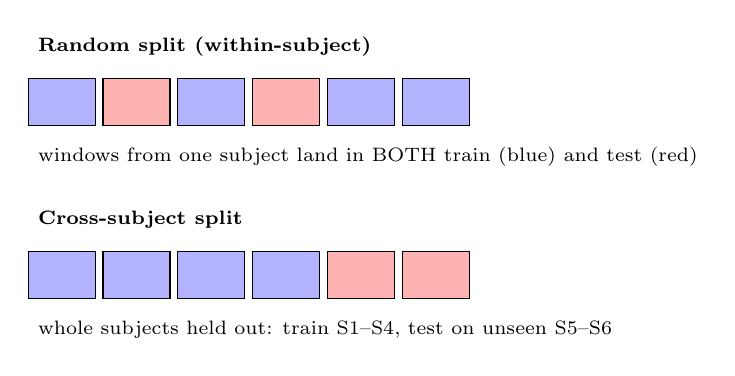
\begin{tikzpicture}[font=\scriptsize]
% within-subject split
\node[anchor=west] at (0,3.5) {\textbf{Random split (within-subject)}};
\foreach \i/\c in {0/blue!30,1/red!30,2/blue!30,3/red!30,4/blue!30,5/blue!30}{
  \fill[\c] (\i*0.95,2.5) rectangle (\i*0.95+0.85,3.1);
  \draw (\i*0.95,2.5) rectangle (\i*0.95+0.85,3.1);
}
\node[anchor=west] at (0,2.1) {windows from one subject land in BOTH train (blue) and test (red)};
% cross-subject split
\node[anchor=west] at (0,1.3) {\textbf{Cross-subject split}};
\foreach \i/\c in {0/blue!30,1/blue!30,2/blue!30,3/blue!30,4/red!30,5/red!30}{
  \fill[\c] (\i*0.95,0.3) rectangle (\i*0.95+0.85,0.9);
  \draw (\i*0.95,0.3) rectangle (\i*0.95+0.85,0.9);
}
\node[anchor=west] at (0,-0.1) {whole subjects held out: train S1--S4, test on unseen S5--S6};
\end{tikzpicture}
\caption{Two ways to split. Top: random split mixes each subject across train/test, so a
model can cheat by identifying the person. Bottom: cross-subject split holds out whole
people, measuring true generalization to new users.}
\label{ch39:fig-cross-subject}
\end{figure}

\begin{connectionbox}
In probability terms (Chapter~42), the \emph{i.i.d.\ assumption} fails here. Windows
from one person are not independent of each other -- they share that person's quirks. The
right unit of independence is the \emph{subject}, not the window, so the right split is
by subject. Get the unit of independence wrong and every confidence interval you compute
is invalid.
\end{connectionbox}

\begin{example}[How big the gap can be]
\label{ch39:ex-gap}
A 1-D CNN on a 6-gesture IMU set might report 97\% accuracy under random splitting and
only 74\% under leave-one-subject-out -- a 23-point drop that is \emph{entirely} an
artifact of how you evaluated, not of any change to the model. The 74\% is the number
that predicts field performance. Gesture papers that report only random-split numbers
are, intentionally or not, overstating real-world accuracy. Always ask which split a
number came from.
\end{example}

\begin{goalbox}
The cross-subject gap is the reason our capstone skips the learned model entirely. Even a
good cross-subject model usually needs a \emph{tiny per-user calibration} -- ask a new
user to perform each gesture three or four times at setup -- to close the gap. But once
you accept a short enrollment, you may as well calibrate \emph{directly}: record each
user's own gesture templates and match against them, no training set required. That is
the path the wrist controller takes. The lesson to carry forward is the enrollment step,
not the classifier: expect a 30-second setup, not a one-size-fits-all model.
\end{goalbox}

\section{Beyond accuracy: confusion and thresholds}
\label{ch39:confusion}

A single accuracy number hides which gestures get mixed up. The \emph{confusion matrix}
counts, for each true gesture (row), how often the model predicted each label (column).
Its diagonal is correct calls; off-diagonal entries are the specific mistakes -- and they
are very useful for design. If ``pinch'' and ``rest'' are confused but everything else is clean,
you learn that your sensor barely sees the pinch, and the fix is better sensing, not a
fancier model.

\begin{figure}[H]
\centering
\begin{tikzpicture}[font=\scriptsize]
\matrix (m) [matrix of nodes, nodes={draw, minimum size=1.0cm, anchor=center},
  column sep=-\pgflinewidth, row sep=-\pgflinewidth]{
   |[fill=green!30]| 41 & 2 & 0 \\
   3 & |[fill=green!30]| 38 & 4 \\
   1 & 9 & |[fill=green!30]| 30 \\
};
\node[above=2pt of m-1-1, anchor=south] {rest};
\node[above=2pt of m-1-2, anchor=south] {wave};
\node[above=2pt of m-1-3, anchor=south] {flick};
\node[left=2pt of m-1-1, anchor=east] {rest};
\node[left=2pt of m-2-1, anchor=east] {wave};
\node[left=2pt of m-3-1, anchor=east] {flick};
\node[above=20pt of m-1-2] {predicted};
\node[rotate=90, left=20pt of m-2-1] {true};
\end{tikzpicture}
\caption{A confusion matrix for three gestures. The diagonal (shaded) is correct; here
``flick'' is most often mistaken for ``wave'' (9 windows), telling us exactly where the
sensor or features fall short.}
\label{ch39:fig-confusion}
\end{figure}

For a controller, you can also tune the \emph{decision threshold}: only emit a MIDI event
when $\max_k \hat{p}_k$ exceeds, say, $0.8$, and otherwise stay silent. This trades a few
missed gestures for far fewer false triggers -- usually the right call for an instrument,
where a spurious note is more jarring than a dropped one.

\section{On-device inference on a microcontroller}
\label{ch39:ondevice}

Training happens on a laptop. \emph{Inference} -- running the trained model on each new
window -- has to happen on the wrist, on a microcontroller (MCU) with maybe 256\,KB of
RAM, a tight cycle budget, and a small battery that has to last through a rehearsal. Three
budgets dominate.

\begin{itemize}
  \item \textbf{Latency.} For a responsive instrument the path from motion to MIDI note
        should stay under roughly $30$\,ms; humans notice audio latency above that. With
        a windowed classifier the window length itself adds delay, so short hops and a
        fast model matter.
  \item \textbf{Memory.} The model's parameters plus activation buffers must fit in
        flash and RAM. A random forest of 100 deep trees can be larger than a small
        quantized CNN; an RBF-SVM must store every support vector. Count bytes early.
  \item \textbf{Energy.} Every multiply costs charge. Fewer parameters and integer
        arithmetic both extend battery life directly.
\end{itemize}

\begin{buildbox}
Concrete tactics that make a model fit on an MCU class like an ARM Cortex-M4:
\begin{itemize}
  \item \textbf{Quantize to int8.} Convert float weights/activations to 8-bit integers
        ($4\times$ smaller, and integer multiply-accumulate is fast). Frameworks like
        TensorFlow Lite for Microcontrollers and CMSIS-NN do this and ship the kernels.
  \item \textbf{Prefer small models.} A 2-layer 1-D CNN with a few thousand parameters,
        or a shallow random forest on $\sim\!15$ features, usually beats a big net once
        you account for the cross-subject gap anyway.
  \item \textbf{Compute features on the MCU.} If you classify hand-crafted features, the
        FFT/energy/zero-crossing code from earlier chapters runs on-device; only the tiny
        classifier needs porting.
  \item \textbf{Measure, don't guess.} Toggle a GPIO pin high at window-start and low
        when the label is ready; read the pulse width on a scope. That is your true
        end-to-end latency.
\end{itemize}
\end{buildbox}

\begin{lstlisting}[language=Python, caption={Laptop side: train, evaluate cross-subject (leave-one-subject-out, not random), and export.}]
import numpy as np
from sklearn.ensemble import RandomForestClassifier
from sklearn.model_selection import LeaveOneGroupOut

X, y, subject = load_windows()          # features, labels, per-window subject id
logo = LeaveOneGroupOut()               # the unit of independence is the SUBJECT
accs = []
for tr, te in logo.split(X, y, groups=subject):
    clf = RandomForestClassifier(n_estimators=50, max_depth=8)
    clf.fit(X[tr], y[tr])
    accs.append(clf.score(X[te], y[te]))
print("cross-subject accuracy:", np.mean(accs), "+/-", np.std(accs))
export_thresholds_to_c(clf)             # emit a small C header of split rules
\end{lstlisting}

\begin{lstlisting}[language=C, caption={MCU side: the per-window inference loop. Read a window, compute a few integer features, run a tiny classifier, emit MIDI above threshold.}]
// runs once per hop (e.g., every 100 ms) inside the main loop
float feat[NF];
extract_features(window, feat);          // mean, var, dominant freq, band energy...
int   gesture; float conf;
classify(feat, &gesture, &conf);         // tiny ported model: tree votes or int8 net
if (conf > 0.80f && gesture != REST)
    midi_send_note(GESTURE_TO_NOTE[gesture]);
\end{lstlisting}

\begin{applicationbox}
The same pattern -- window, feature, tiny model, threshold -- powers a fitness band's
step and activity classifier, a hearing aid's speech-vs-noise switch, a smartwatch's
fall detector, and a keyword-spotting chip that wakes on ``Hey.'' All run inference under
a milliamp on an MCU; all face the same latency/memory/energy triangle. What you learn
for the wrist controller applies to all of these embedded systems.
\end{applicationbox}

\section{Data collection and labeling for a gesture set}
\label{ch39:data}

Models are only as good as their data, and for gestures the data is something \emph{you}
must record -- there is no public dataset for your exact band, electrodes, and gesture
vocabulary. This step is tedious, but it largely determines how well the system works. (Even the
template-matching capstone needs this data discipline -- it just feeds the recordings into
calibration templates instead of into a model fit.)

\paragraph{Choose a gesture set the sensor can resolve.} Before recording a single window, list
the gestures and ask, for each pair, ``what in the signal distinguishes these?'' If the
answer is ``nothing my sensor can see,'' cut one. A good wrist-IMU starter set is
\emph{rest, wave, twist (pronate/supinate), tap, sharp flick} -- all gross motions with
distinct accel/gyro signatures. Resist adding ``point with index finger,'' which the wrist
IMU cannot resolve from a flat hand.

\paragraph{Record many repetitions, many people, many sessions.} The goal is to capture
variation. Collect from at least 8--12 people so cross-subject evaluation has held-out
strangers to test on. Record multiple sessions per person, taking the band off and
re-donning it between sessions, because band placement is one of the biggest sources of
drift -- if the model only ever saw one placement it will fail when the band rotates 1\,cm.

\paragraph{Label cleanly.} Use a cued protocol: a screen prompts ``WAVE'' for two
seconds, the subject performs, you tag those samples. Discard the transition regions at
the start and end of each cue, where the hand is still moving into or out of the gesture
and the label is genuinely ambiguous. Always keep a generous \emph{rest / null} class --
in deployment the hand is at rest the vast majority of the time, and a model that never
learned ``nothing is happening'' will fire constantly.

\begin{trapbox}
Two labeling traps that quietly inflate your accuracy: (1) recording all of one person's
gestures back-to-back in one session, so the model latches onto that session's exact
band placement; and (2) letting windows overlap across the train/test boundary, so a
single gesture's first half trains and its second half tests -- near-duplicate leakage.
Split by subject and by recording, and keep overlapping windows entirely on one side of
the split.
\end{trapbox}

\begin{goalbox}
A realistic first dataset for a learned gesture system: 10 people $\times$ 3 sessions
$\times$ 5 gestures $\times$ 20 repetitions, windowed at 1\,s with 50\% overlap. That is a
few thousand windows -- plenty for a random forest on hand features, marginal for a CNN on
raw windows. If you go the learned route, start with features and a forest, get a clean
cross-subject number, and only reach for a CNN if more data and a richer gesture set
justify it. For the capstone we spend that same recording effort on per-user calibration
templates instead, which sidesteps the cross-subject gap by never training a shared model
in the first place (Section~\ref{ch39:cross-subject}).
\end{goalbox}

\section{Machine Learning on Signals: Decision Boundaries, Latency, and Generalization}
\label{ch39:capabilities-limits}

\subsection{What Machine Learning on Signals Unlocked}
Machine learning replaces hand-tuned thresholds with decision boundaries fit to data:
\begin{itemize}
  \item \emph{Non-linear, multi-modal boundaries:} Kernel SVMs and Random Forests can fit complex non-linear classification regions across heterogeneous inputs --- fusing IMU kinematics with FMG pressures and EMG envelopes without requiring hand-tuned geometric thresholds.
  \item \emph{Principled structural risk minimization:} Vapnik's maximum-margin formulation provides theoretical bounds on generalization error, and the widest-margin boundary gives the most tolerance to sensor jitter.
\end{itemize}

\subsection{Downsides and Limitations}
Machine learning models on embedded signals face practical constraints:
\begin{itemize}
  \item \emph{Embedded memory and compute ceilings:} An RBF kernel SVM with $300$ support vectors in $\R^{15}$ requires $4,500$ floating-point multiplications and $300$ exponential evaluations per classified window. On an ultra-low-power coin-cell microcontroller, this computational footprint quickly drains the battery and risks missing real-time audio deadlines.
  \item \emph{Covariate shift and the cross-subject gap:} Human anatomy varies across arm girth, subcutaneous fat, and muscle recruitment order. A model trained on ten participants can completely misclassify gestures on an eleventh participant, or on the original user after the wristband is taken off and put back on.
  \item \emph{Data collection burdens:} Training complex statistical models demands hundreds of labeled repetitions across multiple days and subjects. For an individual musical controller, a direct 30-second template enrollment often outperforms a complex model with zero training overhead.
\end{itemize}

\subsection{Next: From Statistical Models to Embedded Hardware}
We have now covered the whole signal processing chain: sampling, filtering, spectral analysis, orientation fusion, bio-signal conditioning, and gesture classification. So far, all of it has run in desktop Python notebooks. 

In \textbf{Chapter 40}, we move to physical hardware: \textbf{Embedded DSP on Arduino and Raspberry Pi}. We will trace the evolution of digital signal hardware from the landmark \textbf{TI TMS32010} (1983) to modern \textbf{ARM Cortex-M4 SIMD} processors, work through fixed-point Q-format math, and configure \textbf{ping-pong DMA} buffers to process audio-rate signals with zero CPU jitter.

\section{Exercises}
\label{ch39:exercises}

\begin{exercise}
A logistic-regression gesture detector has $\vec{w}=(2,-1)$ and $b=-1$ over features
$(x_1,x_2)$. (a) Write the decision boundary as a line in the plane. (b) Classify the
window $\vec{x}=(2,1)$: compute $z$, then $\hat{p}=\sigma(z)$, and give the predicted
label at threshold $0.5$. (c) Which side of the boundary does $\vec{w}$ point toward,
positive or negative class?
\end{exercise}

\begin{exercise}
Using the cross-entropy gradient
$\partial L/\partial\vec{w}=\tfrac1N\sum(\hat{p}^{(n)}-y^{(n)})\vec{x}^{(n)}$, explain in
one or two sentences why a correctly and confidently classified example
($\hat{p}\approx y$) contributes almost nothing to the gradient, while a confident
\emph{mistake} contributes a lot. What does this say about which examples drive learning?
\end{exercise}

\begin{exercise}
For a separable two-class problem, an SVM finds margin half-width $1/\norm{\vec{w}}$. If
retraining on more data yields a \emph{larger} $\norm{\vec{w}}$, did the margin get wider
or narrower, and what does that suggest about how separable the new data is?
\end{exercise}

\begin{exercise}
You train a model and observe: training accuracy 99\%, validation accuracy 71\%, test
accuracy 70\%. (a) Name the phenomenon. (b) List three concrete changes that should
narrow the train--validation gap. (c) Why is it reassuring that validation and test
accuracy are close to each other?
\end{exercise}

\begin{exercise}
A colleague reports 96\% gesture accuracy. You ask how they split the data and learn they
pooled all subjects and split windows randomly. Explain precisely what the model may have
learned instead of the gestures, and describe the experiment you would run to find the
number that predicts field performance.
\end{exercise}

\begin{exercise}
From the confusion matrix in Figure~\ref{ch39:fig-confusion}: (a) compute the overall
accuracy. (b) Compute the per-class recall for ``flick'' (fraction of true flicks
correctly labeled). (c) Which single confusion would you attack first, and would you
attack it with a better sensor, better features, or a bigger model? Justify.
\end{exercise}

\begin{exercise}
Explain in your own words why a 1-D convolution layer is ``a stack of FIR filters whose
taps are learned.'' Then state one thing a learned conv kernel can do that a fixed
band-pass cannot, and one thing the fixed band-pass guarantees that the learned kernel
does not.
\end{exercise}

\begin{exercise}
You must fit a classifier in 64\,KB of flash with a 20\,ms latency budget. Compare a
random forest of 100 trees of depth 12, an RBF-SVM with 800 support vectors, and a
quantized 2-layer 1-D CNN with 4{,}000 int8 weights. Estimate the storage of each
(state your assumptions) and argue which is the safest choice and why.
\end{exercise}

\begin{exercise}
Design a cued data-collection protocol for the five-gesture set \{rest, wave, twist, tap,
flick\}. Specify: number of subjects and sessions, repetitions per gesture, window length
and overlap, how you handle the transition regions between cues, and how you will split
the resulting data for a trustworthy cross-subject evaluation.
\end{exercise}

\begin{exercise}
A wrist-IMU gesture system works well in the lab but users complain it misfires while they
walk. (a) Why would walking specifically confuse an accel/gyro gesture model? (b) Propose
two fixes -- one in data collection, one in the runtime decision logic -- and explain what
each one costs.
\end{exercise}

\begin{exercise}
(Feature engineering vs.\ end-to-end representation learning.) Consider an IMU streaming 6 axes ($a_x, a_y, a_z, g_x, g_y, g_z$) at $200\,\text{Hz}$ across a $500\,\text{ms}$ window ($100$ time steps per axis), yielding a raw concatenated vector of dimension $D = 600$.
\begin{enumerate}[label=(\alph*)]
  \item If a wearable training set contains only $N = 300$ labeled gesture repetitions, explain from statistical learning theory why fitting an RBF-kernel SVM directly on raw 600-dimensional vectors is vulnerable to the curse of dimensionality ($D \gg N$).
  \item Suppose you instead extract 8 summary DSP features per axis (mean, variance, peak-to-peak amplitude, zero-crossing rate, spectral centroid, sub-band energies, and dominant DFT peak), reducing dimension from $D = 600$ to $D = 48$. Explain geometrically how this domain-informed projection stabilizes the SVM margin and bounds the generalization error.
  \item Under what concrete conditions regarding training dataset size, user diversity, and microcontroller compute budget would an end-to-end 1-D CNN become superior to hand-crafted DSP features?
\end{enumerate}
\end{exercise}

\begin{exercise}
(Programming.) Using the laptop-side code sketch as a starting point, write a script that
loads windowed features, runs both a random-split and a leave-one-subject-out evaluation
of a random forest, and prints both numbers with their standard deviations. Comment on
the size of the gap you would expect to see and why the leave-one-subject-out number is
the one to trust.
\end{exercise}
